\documentclass[twoside,10pt]{article}
\usepackage{amsmath,amsfonts,amsthm,fullpage}
\usepackage{algorithm}
\usepackage{algorithmic}
\usepackage{graphicx}


\begin{document}

\title{ISYE 6740 Summer 2021\\ Homework 1 (100 points + 2 bonus points)}
%\author{Yao Xie}
\date{}

\maketitle

\vspace{-.5in}

%In this homework, the superscript of a symbol $\text x^i$ denotes the index of samples (not raising to $i$th power); this is a convention in this class. 


\section{Image compression using clustering [60 points]}

In this programming assignment, you are going to apply clustering algorithms for image compression. Your task is implementing \emph{$K$-means} for this purpose.  {\bf It is required you implementing the algorithms yourself rather than calling k-means from a package. However, it is ok to use standard packages such as file i/o,  linear algebra, and visualization.} 


\subsubsection*{Formatting instruction}


\textbf{Input}
\begin{itemize}
  \item \texttt{pixels}: the input image representation. Each row contains one data point (pixel). For image dataset, it contains 3 columns, each column corresponding to Red, Green, and Blue component. Each component has an integer value between 0 and 255.
  \item \texttt{k}: the number of desired clusters. Too high value of $K$ may result in empty cluster error. Then, you need to reduce it.
\end{itemize}

\textbf{Output}
\begin{itemize}
  \item \texttt{class}: cluster assignment of each data point in pixels. The assignment should be 1, 2, 3, etc. For $k = 5$, for example, each cell of class should be either 1, 2, 3, 4, or 5. The output should be a column vector with \texttt{size(pixels, 1)} elements.
  \item \texttt{centroid}: location of $k$ centroids (or representatives) in your result. With images, each centroid corresponds to the representative color of each cluster. The output should be a matrix with $K$ rows and 3 columns. The range of values should be [0, 255], possibly floating point numbers.
\end{itemize}

\subsubsection*{Hand-in}
Both of your code and report will be evaluated. Upload them together as a zip file. In your report, answer to the following questions:
\begin{enumerate}
  \item (20 points) Use $k$-means with squared-$\ell_2$ norm as a metric, for \texttt{GeorgiaTech.bmp} and \texttt{football.bmp} and also choose a third picture of your own to work on. We recommend size of $320 \times 240$ or smaller. Run your $k$-means implementation with these pictures, with several different $k = 2, 4, 8, 16$. How long does it take to converge for each $k$ (report the number of iterations, as well as actual running time)? Please write in your report, and also include the resulted compressed pictures for each $k$.
  \item (20 points) Run your $k$-means implementation (with squared-$\ell_2$ norm) with different initialization centroids. Please test two initialization strategies, compare the results (output image, running time, iterations) and report: (i)
random initialization. Please try multiple time and report the best one (in terms of the image quality).
(ii) poor initialization. Please design your own strategy, explain why it qualifies as a poor initialization, try multiple times, and report the results.
  
  How does this it affect your final result? (We usually randomize initial location of centroids in general.) Please also explain in the report how you initialize the centroid.
   \item (20 points) Now try your $k$-means with the Manhattan distance (or $\ell_1$ distance) and repeat the same steps in Part (1). Please note that the assignment of data point should be based on the Manhattan distance, and the cluster centroid (by minimizing the sum of deviance -- as a result o fusing the Manhattan distance) will be taken as the ``median'' of each cluster. Comment on the difference of image compression results using the two methods.
\end{enumerate}


\subsubsection*{Note}
\begin{itemize}
  \item You may see some error message about empty clusters when you use too large $k$. Your implementation should treat this exception as well. That is, do not terminate even if you have an empty cluster, but use smaller number of clusters in that case.

  \item   We recommend you to test your code with several different pictures so that you can detect some problems that might happen occasionally. 

  \item If we detect copy from any other student's code or from the web, you will not be eligible for any credit for the entire homework, not just for the programming part. Also, directly calling built-in functions or from other package functions is not allowed.
\end{itemize}

\section{Spectral clustering and discover football colleague [40 points + 2 bonus]}

First consider the following simple graph
\begin{center}
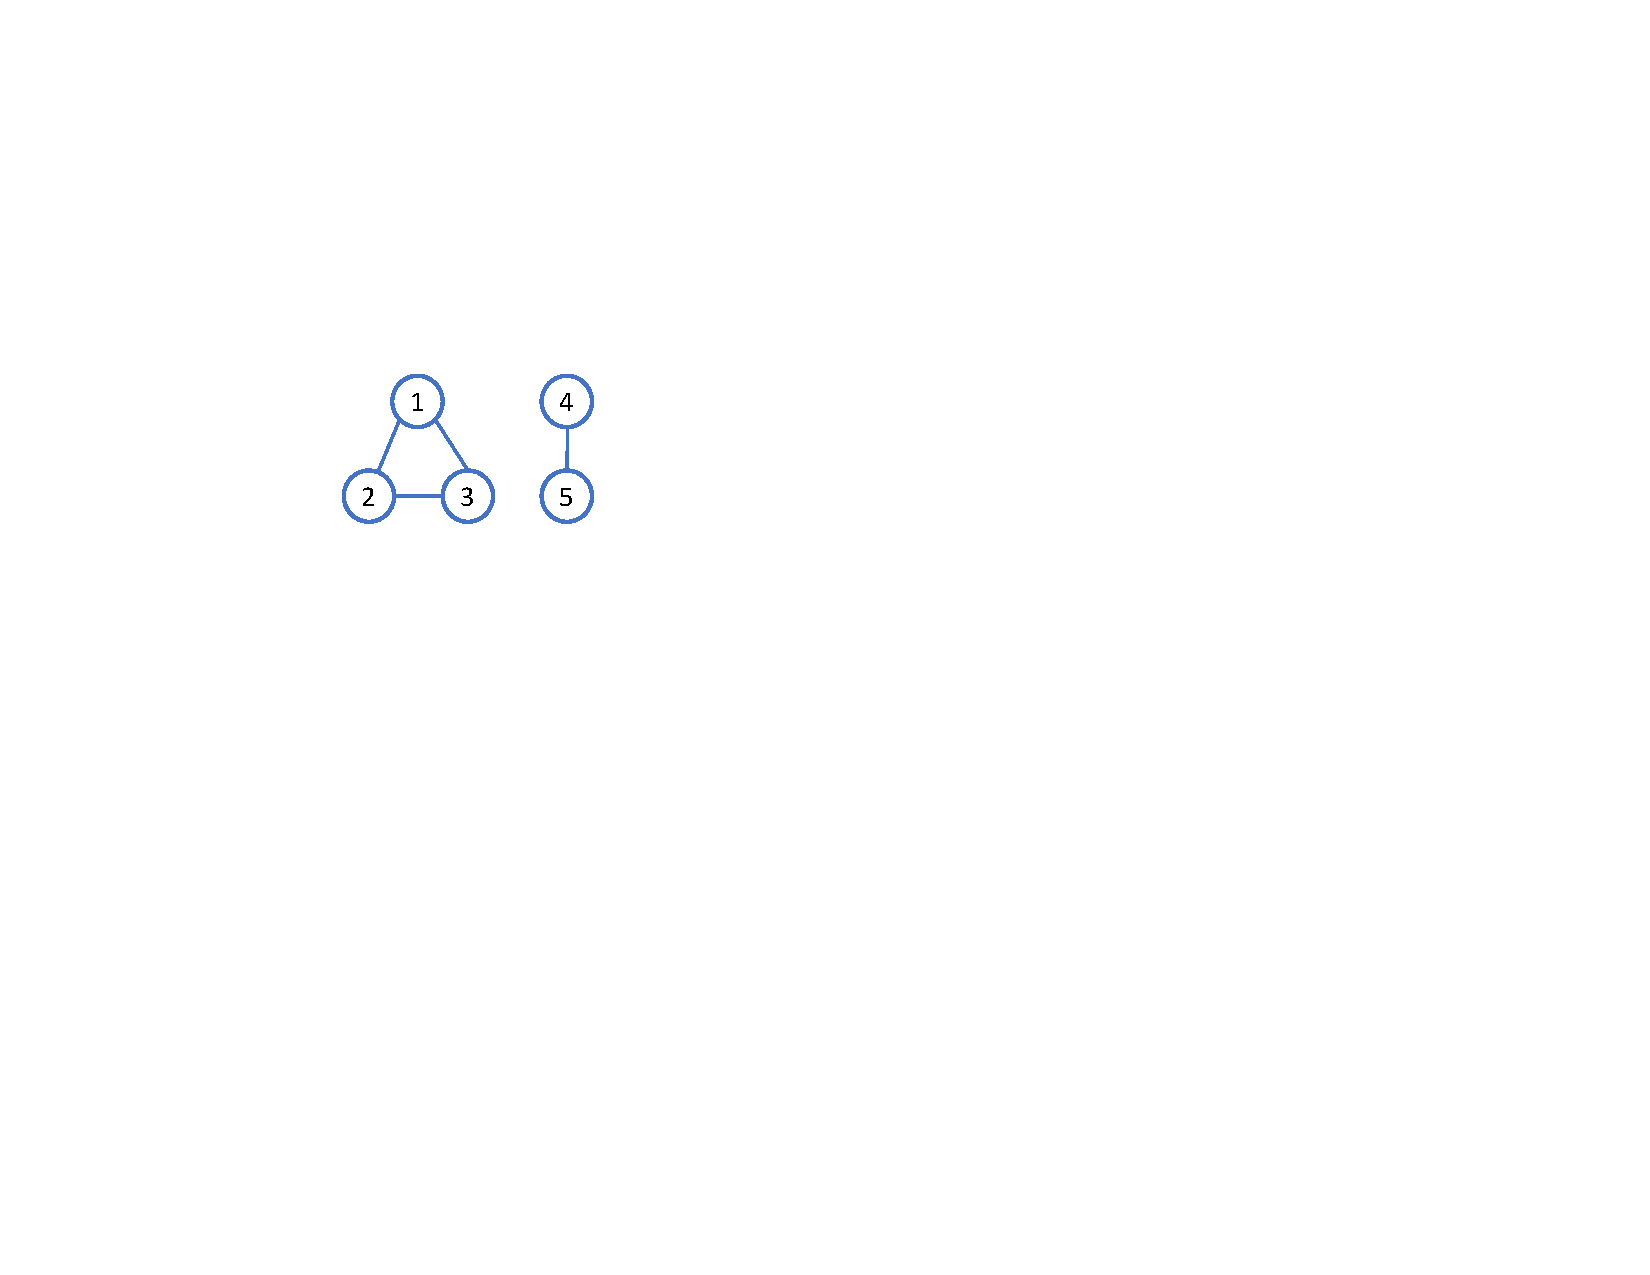
\includegraphics[width = 0.2\textwidth]{plot}
\end{center}
\begin{enumerate}
\item (10 points) Write down the graph Laplacian matrix and find the eigenvectors associated with the zero eigenvalue. Explain how do you find out the number of disconnected clusters in graph and identify these disconnected clusters using these eigenvectors.
\end{enumerate}

Now consider the football league example in the ``spectral clustering'' lecture. Use the data provided there (in demo, \textsf{play\_graph.txt}, \textsf{nodes.csv} and \textsf{edges.csv}) for this question. Implement the spectral clustering algorithm yourself (you can borrow the idea from demo code, in particular, regarding importing data, read data etc.) 

\begin{enumerate}
\item[2.] (10 points) For the graph Laplacian matrix and perform eigedecomposition on it. Plot the eigenvalues (ranked from the largest to the smallest), and based on the plot explain approximately how many clusters you believe there are and why.

\item[3.] (15 points) Now perform spectral clustering, using $k = 5$, $k = 7$, $k=10$, and your choice of $k$ (based on your answer in Part (2). Report the size of the largest cluster and the smallest cluster based on your result for each $k$. Report the results for $k=10$ by listing the teams and which cluster they belong to (you can either include a table in your solution, or upload a file or spreadsheet that include your result).  

\item[4.] (5 points) Now run the algorithm a few times for $k=10$. You may notice the results are slightly different - please explain why. Also check which clusters that ``Georgia Tech'', ``Georgia State'', and ``Georgia'' (UGA) are in. Are they always in the same cluster or not - please explain your reasoning. 

\item[5.] (Bonus, 2 points.) Please report what else you can discover from this data analysis and results. Try to be creative.

\end{enumerate}

\end{document}
